% !TeX root = ../thesis.tex
\subsection{Meshing examples}
\paragraph{}
In this section, some other mesh examples with irregular geometric boundaries are considered.
Fig.~\ref{oct_ex:mesh_spinner} shows the mesh generated for a spinner with a CAD input illustrated in Fig.~\ref{oct_ex:mesh_spinner_cad}.
Fig.~\ref{oct_ex:mesh_sphnix} shows the mesh generated for an Egypt Sphinx with a CAD input plotted in Fig.~\ref{oct_ex:mesh_sphnix_cad}

\begin{figure}
    \centering
    \scalebox{0.25}{
        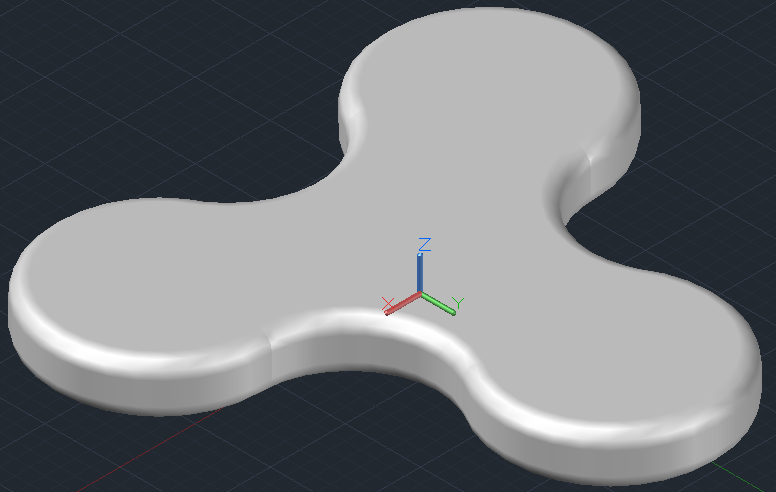
\includegraphics{octree/ex_images/spinner_cad.png}
    }
    \caption[CAD design for spinner]{CAD design for the spinner}
    \label{oct_ex:mesh_spinner_cad}
\end{figure}

\begin{figure}
    \centering
    \begin{subfigure}[b]{0.49\linewidth}
        \centering
        \scalebox{0.25}{
            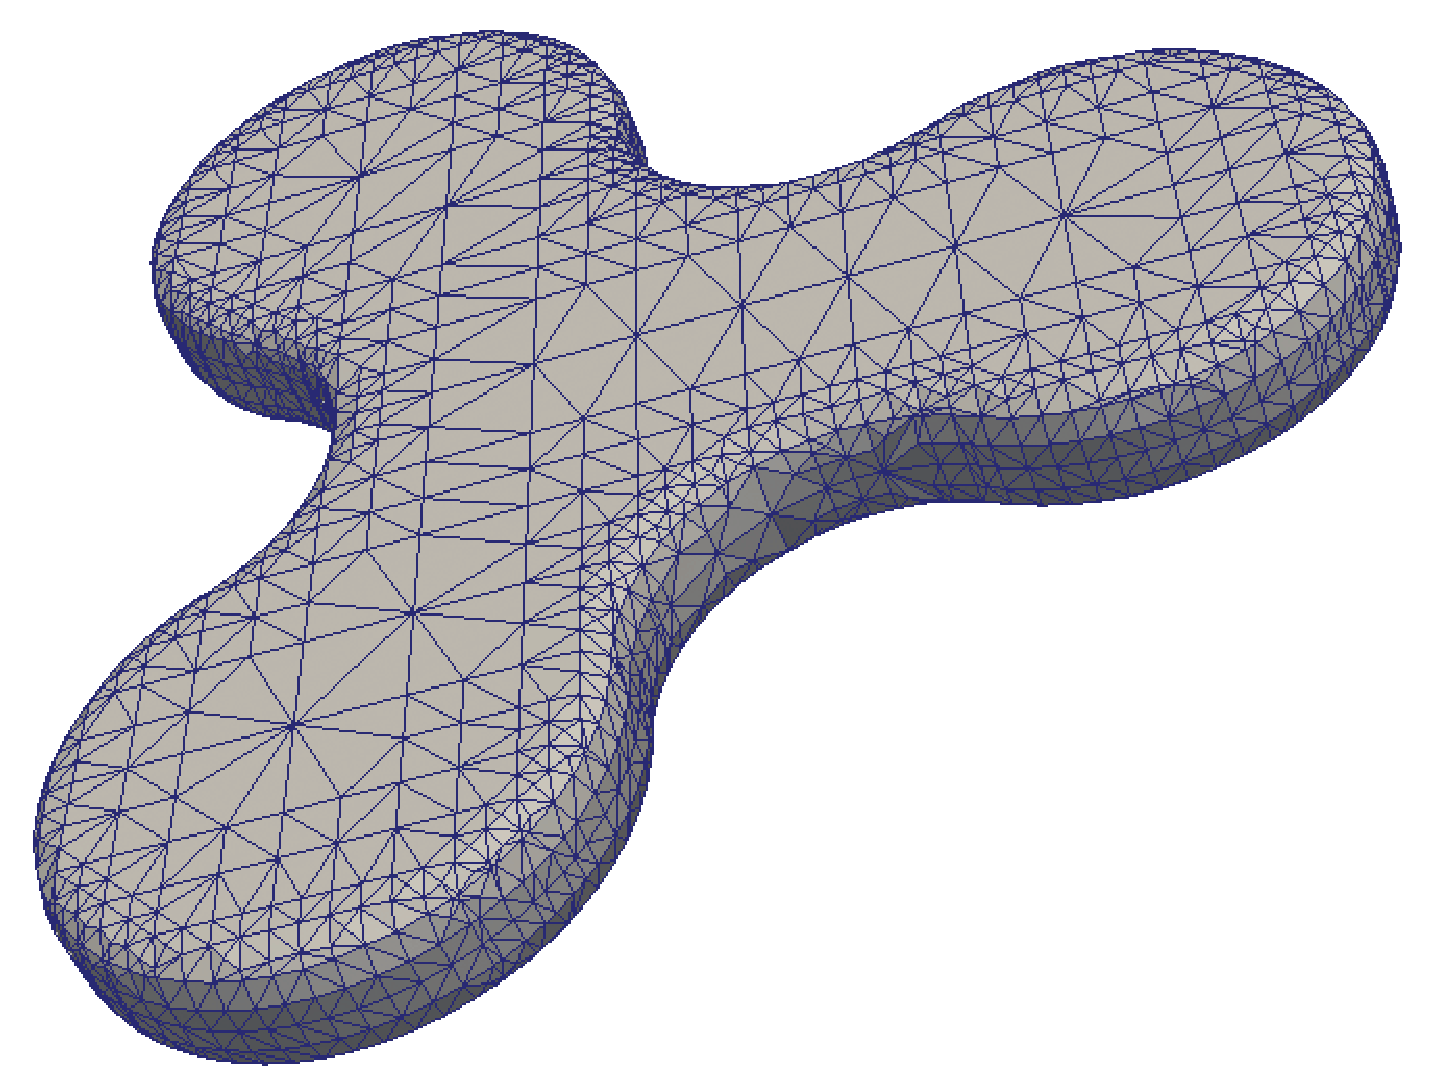
\includegraphics{octree/ex_images/spinner_full.eps}
        }
    \end{subfigure}
    \begin{subfigure}[b]{0.49\linewidth}
        \centering
        \scalebox{0.25}{
            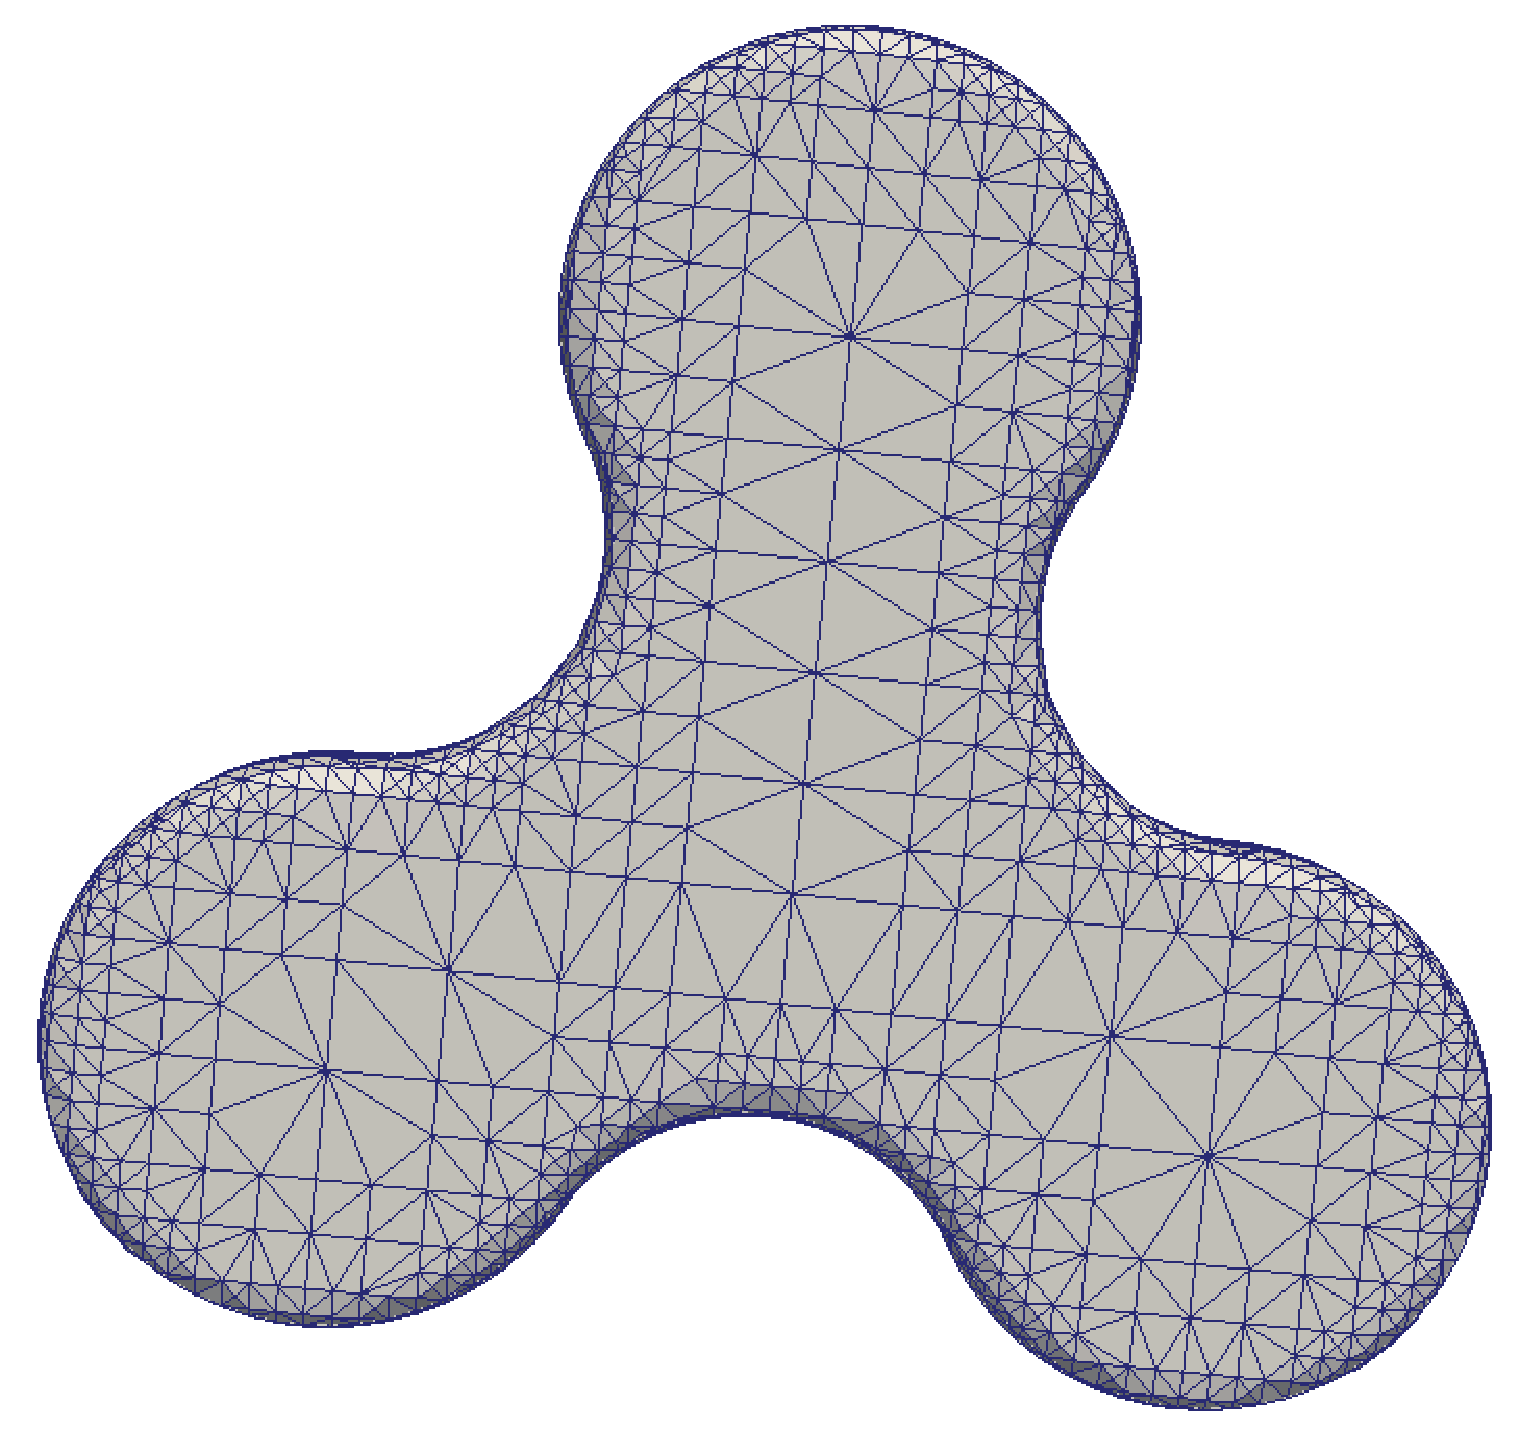
\includegraphics{octree/ex_images/spinner_full_top.eps}
        }
    \end{subfigure} \\
    \begin{subfigure}[b]{0.49\linewidth}
        \centering
        \scalebox{0.25}{
            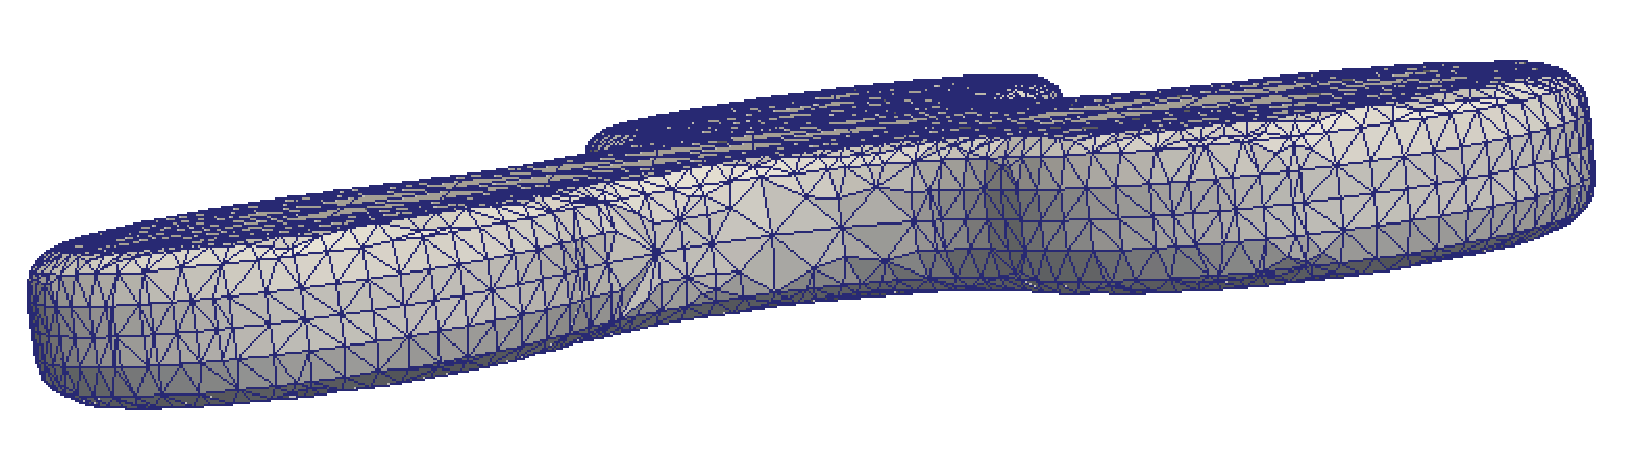
\includegraphics{octree/ex_images/spinner_full_side.eps}
        }
    \end{subfigure}
    \begin{subfigure}[b]{0.49\linewidth}
        \centering
        \scalebox{0.25}{
            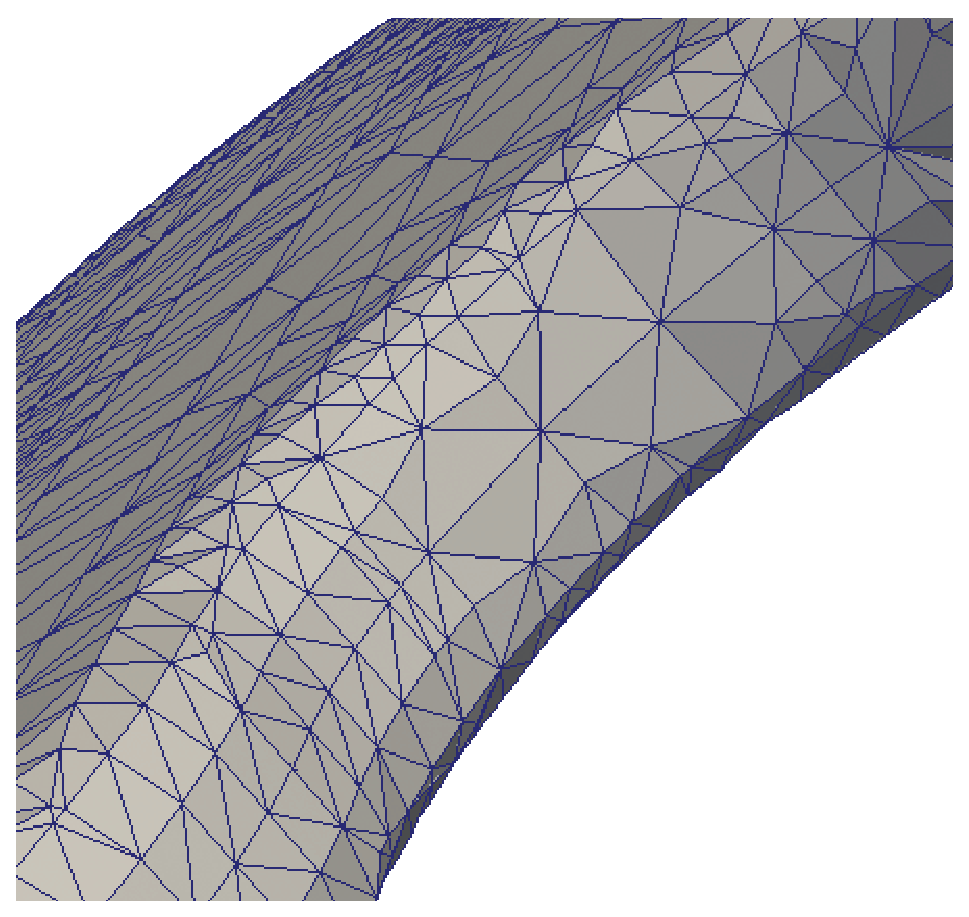
\includegraphics{octree/ex_images/spinner_part.eps}
        }
    \end{subfigure}
    \caption[Mesh for the spinner]{Mesh for the spinner}
    \label{oct_ex:mesh_spinner}
\end{figure}

% ---- %

\begin{figure}
    \centering
    \scalebox{0.4}{
        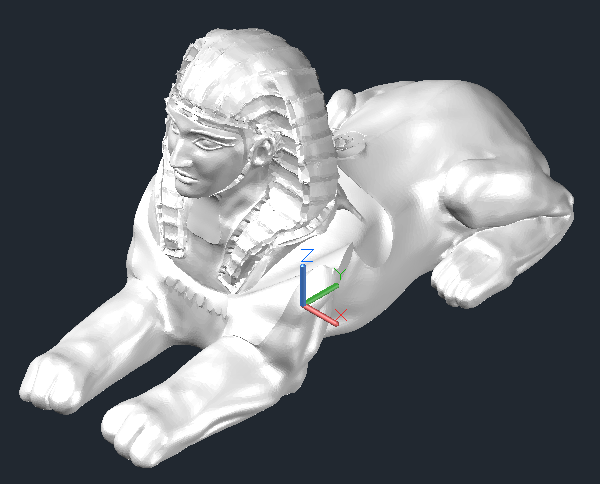
\includegraphics{octree/ex_images/sphnix_cad.png}
    }
    \caption[CAD design for the Egypt Sphinx]{CAD design for the Egypt Sphinx}
    \label{oct_ex:mesh_sphnix_cad}
\end{figure}

\begin{figure}
    \centering
    \begin{subfigure}[b]{0.49\linewidth}
        \centering
        \scalebox{0.25}{
            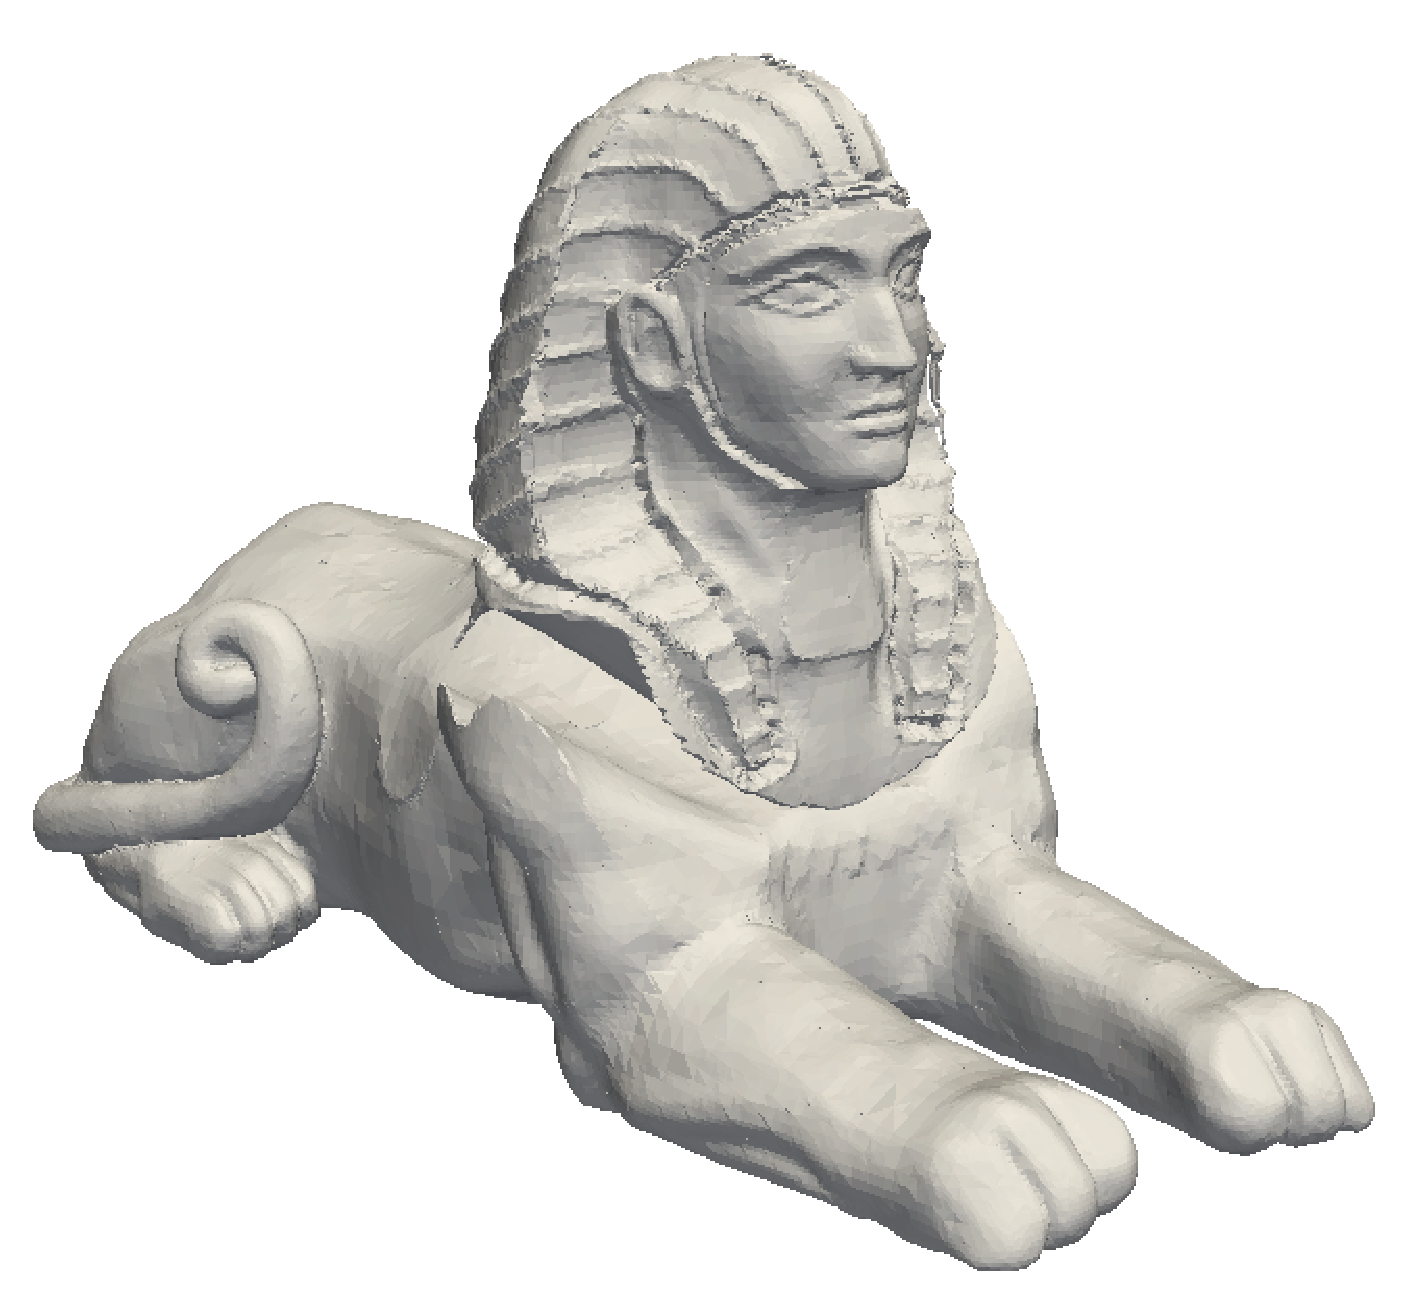
\includegraphics{octree/ex_images/sphnix_full.eps}
        }
    \end{subfigure}
    \begin{subfigure}[b]{0.49\linewidth}
        \centering
        \scalebox{0.25}{
            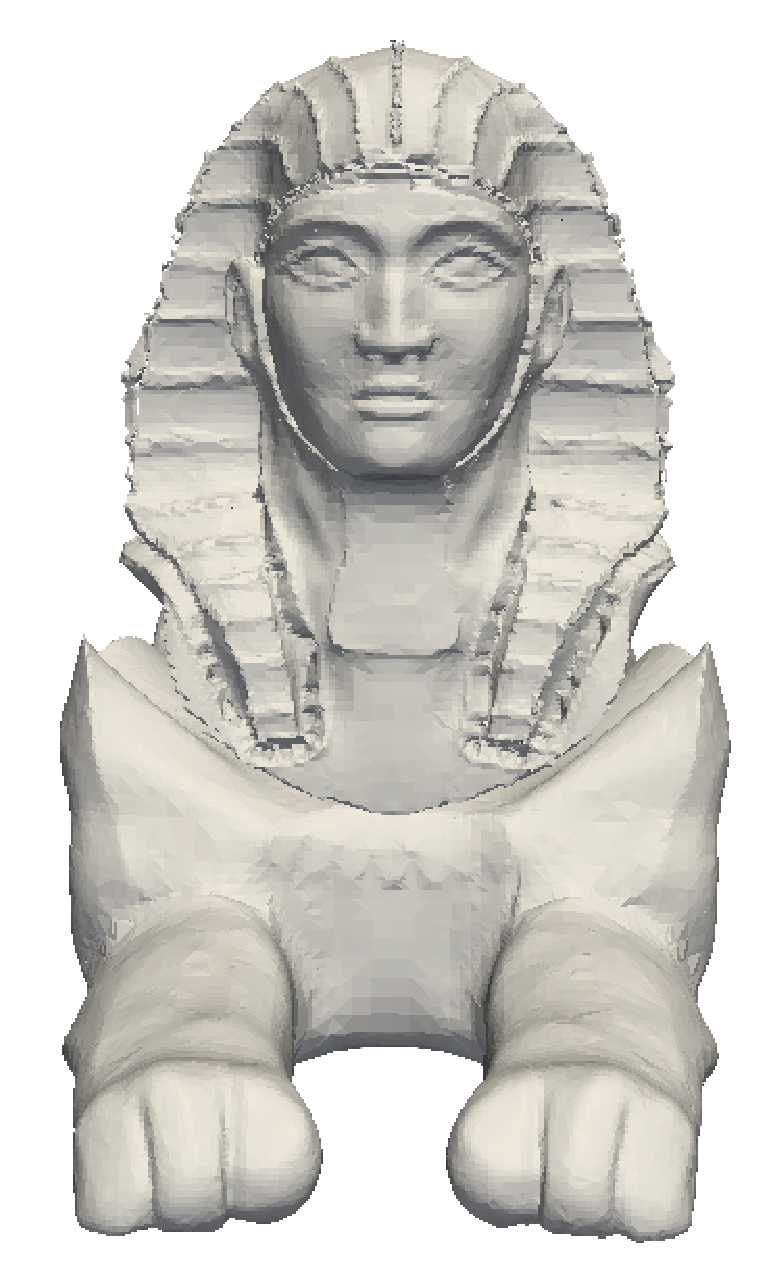
\includegraphics{octree/ex_images/sphnix_front.eps}
        }
    \end{subfigure} \\
    \begin{subfigure}[b]{0.49\linewidth}
        \centering
        \scalebox{0.2}{
            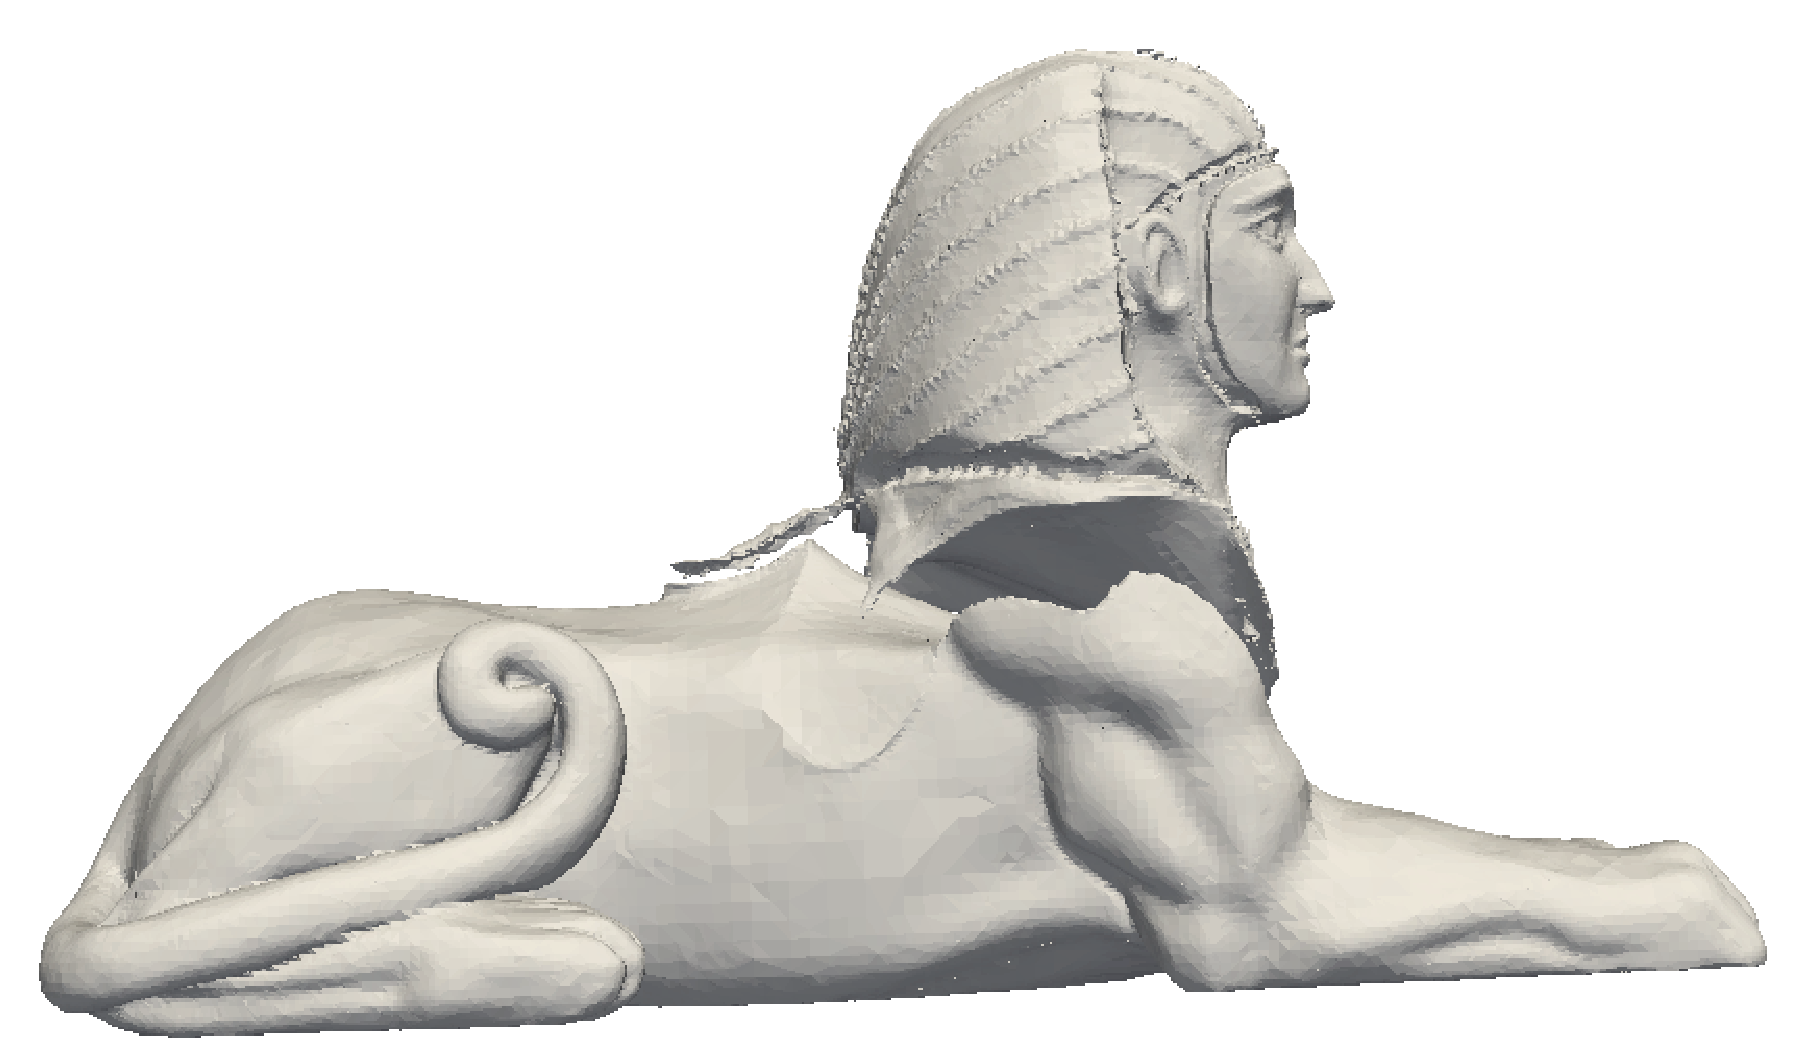
\includegraphics{octree/ex_images/sphnix_side.eps}
        }
    \end{subfigure}
    \begin{subfigure}[b]{0.49\linewidth}
        \centering
        \scalebox{0.125}{
            \includegraphics{octree/ex_images/sphnix_edges.eps}
        }
    \end{subfigure}\\
    \begin{subfigure}[b]{1\linewidth}
        \centering
        \scalebox{0.3}{
            \includegraphics{octree/ex_images/sphnix_internal.eps}
        }
    \end{subfigure}
    \caption[Mesh for the Egypt Sphinx]{Mesh for the Egypt Sphinx}
    \label{oct_ex:mesh_sphnix}
\end{figure}